\begin{figure}[t]
\centering
    \begin{subfigure}[t]{0.24\textwidth}
        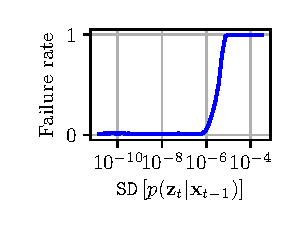
\includegraphics[width=\textwidth]{figures/bot_rate/bot_rate.pdf}
        \vspace{-0.8cm}
        \caption{}
        \label{fig:wormsim:bot_rate}
    \end{subfigure}%
    ~%
    \begin{subfigure}[t]{0.24\textwidth}
        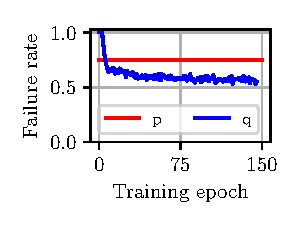
\includegraphics[width=\textwidth]{figures/bot_rate/wormsim_nf_bot_rate.pdf}
        \vspace{-0.8cm}
        \caption{}
        \label{fig:wormsim:bot_nf_rate}
    \end{subfigure}
\vspace{-0.5cm}
\caption{Results from the WormSim example introduced in Section \ref{sec:sub:wormsim}.
\ref{fig:wormsim:bot_rate} shows the rate at which the simulator fails increases sharply as a function of the standard deviation of the applied perturbation. 
\ref{fig:wormsim:bot_nf_rate} shows the reduction in rejections during training.
}
\label{fig:bot}
\end{figure}